%\customlink{Magnetic_anisotropy_and_domains}
\chapter {Magnetic anisotropy and domains}
\label{sect:anisintro}




Rocks often contain assemblages of  ferromagnetic minerals dispersed within a matrix of diamagnetic and paramagnetic minerals.  In later chapters we will be concerned with the magnetization of  these assemblages, but  here we continue our investigation of the behavior of individual particles.   
In Chapter 3 we learned that in some crystals electronic spins work in concert to create a spontaneous magnetization that remains in the absence of an external field.  The basis of paleomagnetism is that these ferromagnetic particles carry the record of ancient magnetic fields.  What allows the magnetic moments to come into equilibrium with the geomagnetic field and then what fixes that equilibrium magnetization into the rock so that we may measure it millions or even billions of years later?  We will begin to answer these questions over the next few chapters.  

We will start  with the second part of the question: what fixes magnetizations in particular directions?     A basic principle is that  ferromagnetic particles have various contributions to the magnetic energy which controls their magnetization.   No matter how simple or complex the combination of energies may become, the grain will seek the configuration of magnetization which minimizes its total energy.  The short answer to our question is that certain directions within magnetic crystals are at lower energy than others.  To shift the magnetization from one ``easy'' direction to another requires energy.  If the barrier is high enough, the particle will stay magnetized in the same direction for very long periods of time -- say billions of years.  In  this chapter we will address the causes and some of the consequences of  these energy barriers for the magnetization of rocks.  Note that in this chapter we will be dealing primarily with energy densities (volume normalized energies), as opposed to energy and will distinguish the two by the convention that energies are given with the symbol $E$ and energy densities with $\epsilon$.    

 In Chapter 6,  we will  discuss the behavior of common magnetic minerals, but to develop the general theory, it is easiest to focus on  a single mineral.  We choose here the most common one, magnetite.  It has a simple, cubic structure and has been the subject intensive study.  However, we will occasionally  introduce concepts appropriate for other magnetic minerals where appropriate.  
 
The simplest permanently magnetized  particles are quasi-uniformly magnetized.  These so-called
 \index{magnetic!domains}%
\index{single domain}%
 {\it single domain} (SD)
particles  have spins that act in concert,  staying as parallel (or anti-parallel) as possible.  As particles get larger, the external energy can be  minimized by allowing neighboring spins to diverge somewhat from strict parallelism; these particles are referred to as {\it pseudo-single domain} or PSD.
  \index{pseudo-single domain}
    Eventually, the spins organize themselves into regions with quasi-uniform magnetization (magnetic domains)
  \index{multi-domain}%
\index{magnetic!domains}%
separated by domain walls and are called {\it multi-domain} (MD)  particles.   These more complicated spin structures are very difficult to model and most paleomagnetic theory is based on the single domain approximation.  Therefore we begin with a  discussion of the energies of uniformly magnetized (single-domain) particles.  

\begin{figure}[htb]
%\epsfxsize 15cm
%\centering \epsffile{EPSfiles/magnetite.eps}
\centering  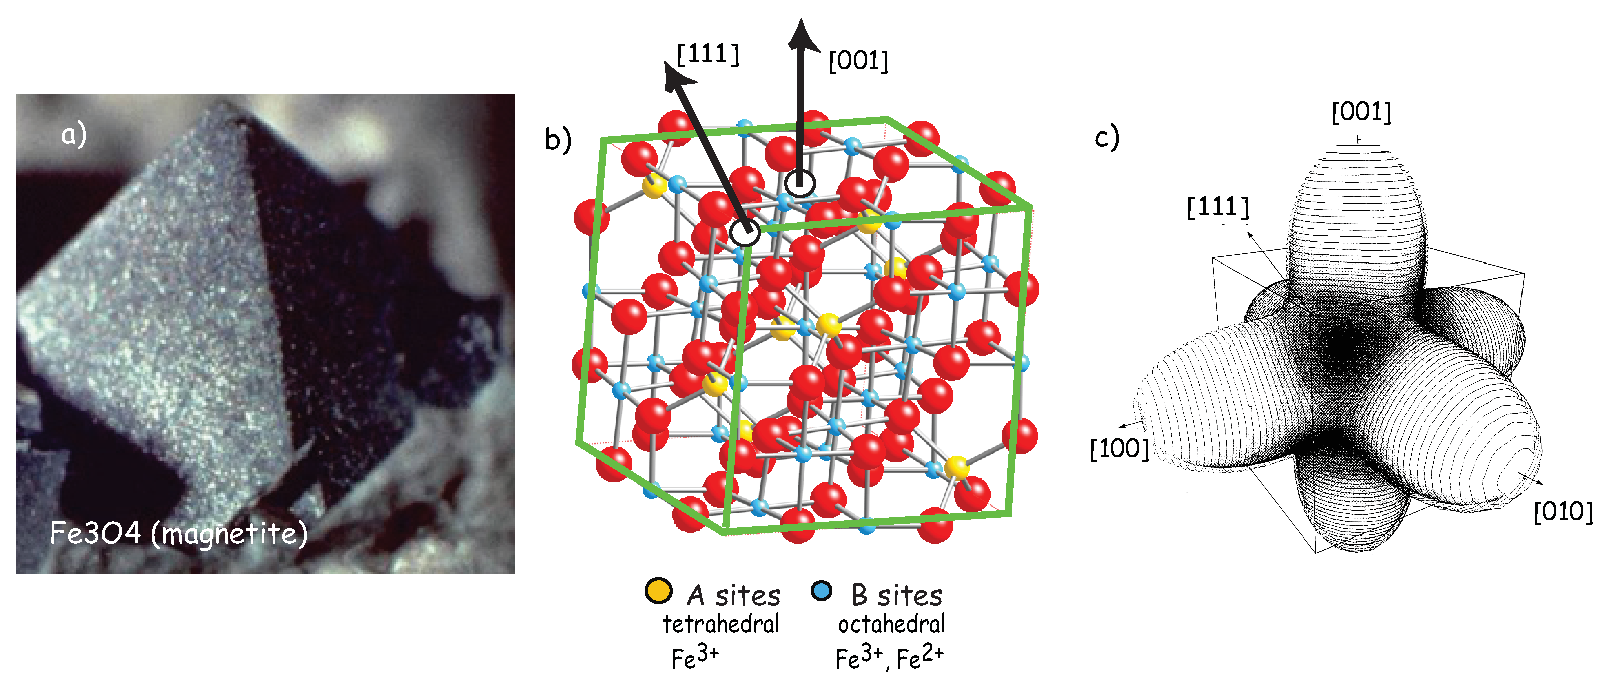
\includegraphics[width=15 cm]{EPSfiles/magnetite.eps}
\caption{a) A magnetite octahedron. [Photo of Lou Perloff in The Photo-Atlas of Minerals.]  b) Internal crystal structure.  Directions of the body diagonal ([111] direction) and orthogonal to the cubic faces ([001] direction)  are shown as arrows.   Big red dots are the oxygen anions.  The blue dots are iron cations in octahedral coordination and the yellow dots are in tetrahedral coordination.  Fe$^{3+}$ sits on the A sites and Fe$^{2+}$ and Fe$^{3+}$ sit on the B sites. c) Magnetocrystalline anisotropy energy as a function of direction within a  magnetite  crystal at room temperature.  The easiest direction to magnetize (the direction with the lowest energy -- note dimples in energy surface) is along the body diagonal (the [111] direction). [Figure from Williams and Dunlop, 1995.]    }
\label{fig:magnetite}
\end{figure}
\nocite{williams95}


 
\section{The magnetic energy of particles}


\index{magnetic!energy!exchange}
\subsection {Exchange energy}
\label{sect:exchange}

We learned in Chapter 3 that some crystalline states are capable of ferromagnetic behavior because of quantum mechanical considerations. Electrons in neighboring orbitals in certain crystals ``know" about each other's spin states.  In order to avoid  sharing the same orbital with the same spin (hence having the same quantum numbers -- not allowed by Pauli's exclusion principle), electronic spins in such crystals act in a coordinated fashion.  They will be either aligned parallel or antiparallel according to the details of the interaction.     This 
{\it exchange energy density} ($\epsilon_e$) is the source of spontaneous magnetization and is given for a pair of spins by:

$$\epsilon_e = -2J_e\S_i \cdot \S_j,
$$
\noindent where $J_e$ is the
\index{magnetic!energy!exchange!integral}
{\it exchange integral} and $\S_i$ and $\S_j$ are spin vectors.  Depending on the details of the crystal structure (which determines the size and sign of the exchange integral), exchange  energy is at a minimum when electronic spins are aligned parallel or anti-parallel.    

We define here a parameter that we will use later: the 
\index{magnetic!energy!exchange!constant}
{\it exchange constant} $A=J_eS^2/a$ where $a$ is the interatomic spacing. $A$ = 1.33 x 10$^{-11}$ Jm$^{-1}$ for magnetite, a common magnetic mineral.   

Recalling the discussion in Chapter 3, while $s$ orbitals which are spherical, the $3d$ electronic orbitals ``poke'' in certain directions.  Hence spins in  some directions within crystals  will be easier to coordinate than in others.   We can illustrate this using the example of magnetite, a common magnetic mineral (Figure~\ref{fig:magnetite}a).  
\index{magnetite}
Magnetite octahedra (Figure~\ref{fig:magnetite}a), when viewed at the atomic level (Figure~\ref{fig:magnetite}b) are composed of one ferrous (Fe$^{2+}$)  cation, two ferric (Fe$^{3+}$) cations  and four O$^{2-}$ anions.  Each oxygen anion shares an electron with two neighboring cations in a covalent bond.  

   In Chapter 3 we mentioned that in some crystals, spins are aligned anti-parallel, yet there is still a net magnetization, a phenomenon we called
   \index{ferrimagnetism}
ferrimagnetism.  This can arise from the fact that not all cations have the same number of unpaired spins.  Magnetite, with its  ferrous (4 $m_b$) and ferric (5 $m_b$) states is a good example.   There are three iron cations in a magnetite crystal giving a total of 14 $m_b$ to play with.    Magnetite is very magnetic, but not that magnetic!   From Figure~\ref{fig:magnetite}b we see that the ferric ions all sit on the tetrahedral (A) lattice sites and there are equal numbers of ferrous and ferric ions sitting on the octahedral (B) lattice sites.  The unpaired spins of the cations in the A and B lattice sites are aligned anti-parallel to one another because of \index{superexchange}
superexchange (Chapter  3)  so we have 9 $m_b$ on the B sites minus 5 $m_b$ on the A sites for a total of 4 $m_b$ per unit cell of magnetite.  




   
   \subsection {Magnetic moments and external fields}

We know from experience that there are energies associated with magnetic fields.  Just as a mass has a potential energy when it is placed in the gravitational field of another mass, a magnetic moment has an energy when it is placed in a magnetic field.  We have seen this energy briefly in Sections~\ref{sect:Me} and Equation~\ref{eq:Em}.  This energy has many names  (magnetic energy, magnetostatic energy, Zeeman energy, etc.).  Here we will work with  the  volume normalized  {\it magnetostatic interaction energy density} ($\epsilon_m$).  This energy density essentially represents the interaction between the magnetic lines of flux and the magnetic moments of the electronic spins.  It is  energy that aligns magnetic compass needles  with the ambient magnetic field.  We find the  volume normalized form (in units of Jm$^{-3}$) by  substituting  $|\M|=|\m|v^{1\over2}$ (see Chapter 1) into Equation~\ref{eq:Em}:

\begin{equation}
\epsilon_m = - \M \cdot \B.
\label{eq:Em1}
\end{equation}

\noindent 
 $\epsilon_m$  is at a minimum when the magnetization $\M$ is aligned with the field $\B$.    Single-domain particles have a quasi-uniform magnetization and the application of a magnetic field does not change the net magnetization, which remains at saturation ($M_s$).  The  direction of all the magnetic spins could swing coherently toward the applied field.    Yet the magnetizations in many particles do not rotate freely toward the magnetic field (or we would not have paleomagnetism!).  There is another contribution to the energy of the magnetic particle  associated with the  magnetic crystal itself.  This energy depends on the direction of magnetization in the crystal -- it is anisotropic -- and  is called
 \index{magnetic!anisotropy energy}
 {\it anisotropy energy}.  Anisotropy energy creates barriers to free rotation of the magnetization within the magnetic crystal, which  lead to energetically preferred directions for the magnetization within individual single-domain grains.  
 
 There are many causes of   anisotropy energy.
 The most important ones derive from the details of crystal structure 
 \index{magnetic!anisotropy energy!magnetocrystalline}
 {\it (magnetocrystalline anisotropy energy)},  the state of stress within the particle {\it (magnetostriction)}, and  the shape of the particle,
 \index{magnetic!anisotropy energy!shape}
  {\it (shape anisotropy)}.  We will consider these briefly in the following subsections. 

 \begin{figure}[htb]
%\epsfxsize 11cm
%\centering \epsffile{EPSfiles/K-T.eps}
\centering  \includegraphics[width=11 cm]{EPSfiles/K-T.eps}
\caption{Variation of $K_1$ and $K_2$ of magnetite as a function of temperature.  Solid lines are data from Syono and Ishikawa (1963). Dashed lines are data from Fletcher and O'Reilly (1974).}
\label{fig:K-T}
\end{figure}
\nocite{syono63} \nocite{fletcher74}

\subsection {Magnetocrystalline anisotropy energy}  
\label{sect:K1}

For equant single-domain particles or particles with low saturation magnetizations,  the crystal structure dominates the magnetic energy. 
\index{magnetic!anisotropy energy!magnetocrystalline}
\index{easy directions}
In such cases, the so-called  {\it easy directions} of magnetization are crystallographic directions along which magnetocrystalline energy is at a minimum.    
 The energy surface shown in Figure~\ref{fig:magnetite}c  represents  the magnetocrystalline anisotropy energy density, $\epsilon_a$ for magnetite at room temperature.   The highest energy bulges are in directions perpendicular to the cubic faces ([001,  010, 100]).  The lowest energy dimples are  along the body diagonals ([111]).    Magnetite (above about 120K) has a cubic structure   with direction cosines  $\alpha_1, \alpha_2, \alpha_3$.  These direction cosines are the angles between a given direction and  the crystallographic axes [100, 010, 001] -- see Appendix~\ref{app:dircosines} for review of direction cosines).  For such a crystal the magnetocrystalline anisotropy energy density is given by:

\begin{equation}
\epsilon_a = K_1(\alpha_1^2 \alpha_2^2 + \alpha_2^2\alpha^2_3 + \alpha_3^2\alpha_1^2) + K_2\alpha_1^2\alpha_2^2\alpha_3^2,
\label{eq:xtalline}
\end{equation}

\noindent where $K_1$ and $K_2$ are empirically determined {\it magnetocrystalline anisotropy constants}.    In the case of (room temperature) magnetite, $K_1$ is -1.35 x 10$^4$ Jm$^{-3}$.  Note that the units of the $K_i$ are in Jm$^{-3}$, so $\epsilon_a$ is in units of energy per unit volume (an energy density).  
If you work through the magnetocrystalline equation, you will find  $\epsilon_a$ is zero parallel to the [100] axis, $K_1/4$ parallel to the [110] and $K_1/3+K_2/27$ parallel to the [111] direction (the body diagonal).    So when $K_1$ is negative,  the [111] direction (body diagonal) has the minimum energy.     This is the reason that there is a dimple in the energy surface along that direction in Figure~\ref{fig:magnetite}c.  



As a consequence of the magnetocrystalline anisotropy energy,   once the magnetization is aligned with an easy direction, work must be done to change it.    In order to switch from one easy axis to another (e.g. from one direction along the body diagonal to the opposite), the magnetization has to traverse  a path over an energy barrier which is the difference between the energy in the easy direction and that in the intervening hard direction.  In the case of magnetite at room temperature, we have this energy barrier as $\epsilon$[111]-$\epsilon$[110] or to first order $K_1/3 - K_1/4 = K_1/12$.  

 \begin{figure}[htb]
%\epsfxsize 12cm
%\centering \epsffile{EPSfiles/verwey.eps}
\centering  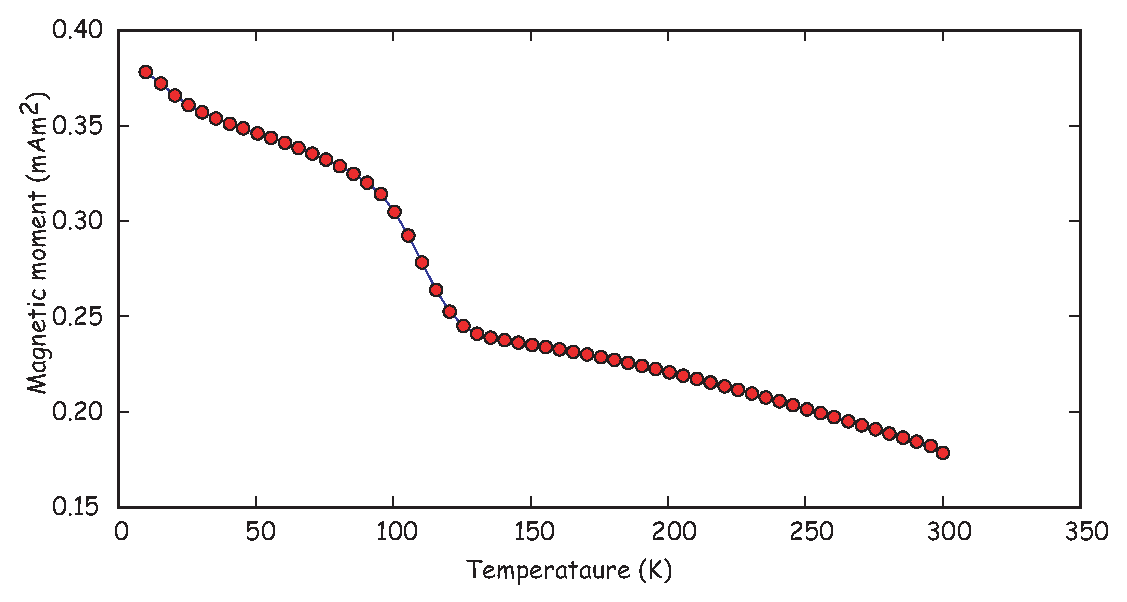
\includegraphics[width=12 cm]{EPSfiles/verwey.eps}
\caption{Magnetization curve for magnetite as a function of temperature.  The specimen was placed in a very large field, cooled to near absolute zero, then warmed up.  The magnetization was measured as it warmed.  When it goes through the Verwey transition ($\sim$110 K), a fraction of the magnetization is lost. Data downloaded from ``w5000'' in the  \href{http://www.irm.umn.edu/bestiary}{Rock magnetic Bestiary} collection at the Institute for Rock Magnetism.}
\label{fig:verwey}
\end{figure}



Because electronic interactions depend heavily on inter atomic spacing, 
\index{magnetic!anisotropy energy!magnetocrystalline}
magnetocrystalline anisotropy constants are a strong function of temperature (see Figure~\ref{fig:K-T}).    In magnetite, $K_1$ changes sign at a temperature known as the 
\index{isotropic point}
{\it isotropic point}.  At the isotropic point, there is no large magnetocrystalline anisotropy.  The large energy barriers that act to keep the magnetizations parallel to the body diagonal are gone and the spins can wander more freely through the crystal.  Below the isotropic point, the energy barriers rise again, but with a different topology in which the crystal axes are the energy minima and the body diagonals are the high energy states.    
 



At room temperature, electrons hop freely between the ferrous and ferric ions on the B lattice sites, so there is no order.  Below about 120 K, there is an ordered arrangement of the ferrous and ferric ions.  Because of the difference in size between the two, the lattice of the unit cell becomes slightly distorted  and becomes monoclinic instead of cubic.  This transition occurs at what is is known as the
\index{Verwey transition}
 {\it Verwey temperature} ($T_v$).   Although the isotropic point (measured magnetically) and the Verwey transition (measured electrically)  are separated in temperature by about 15$^{o}$, they are related phenomena (the ordering and electron hopping cause the change in $K_1$).   

The change in magnetocrystalline anisotropy at low temperature can have a profound effect on the magnetization.  In Figure~\ref{fig:verwey} we show a typical (de)magnetization curve for magnetite taken from the ``Rock magnetic bestiary'' web site maintained at  the Institute for Rock Magnetism: \url{http://irm.umn.edu/bestiary}.  There is a loss of magnetization at around 100 K.  This loss is the basis for 
\index{demagnetization!low-temperature}
{\it low-temperature demagnetization} (LTD).  However, some portion of the magnetization always remains after low temperature cycling (called the {\it low temperature memory}), so the general utility of LTD may be limited.



Cubic symmetry (as in the case of  magnetite) is just one of many types of crystal symmetries.    One other very important form is the uniaxial symmetry which can arise from crystal shape or structure.  The energy density for uniaxial magnetic anisotropy is:

\begin{equation}
\epsilon_a  = K_{u1} sin^2 \theta + K_{u2} \sin^4 \theta + ...
\label{eq:Ku}
\end{equation}

\noindent Here the magnetocrystalline constants have been designated $K_{u1}, K_{u2}$ to distinguish them from $K_1, K_2$ used before.  
In this equation, when the largest
\index{magnetic!anisotropy energy!uniaxial}
{\it uniaxial anisotropy constant},  $K_{_u1}$, is negative, the magnetization is constrained to lie perpendicular to the axis of symmetry.  When $K_{u1}>0$, the magnetization lies parallel to it. 

An example of a mineral dominated by uniaxial symmetry is hematite, a mineral with hexagonal crystal symmetry.  The magnetization of hematite is quite complicated, as we shall learn in Chapters 6 and 7, but one source is  magnetization is 
\index{spin-canting}
spin-canting (see Chapter 3) within the basal plane of the hexagonal crystal.  Within the basal plane, the anisotropy constant is very low and the magnetization wanders fairly freely.  However, the anisotropy energy away from the basal plane is strong, so the magnetization is constrained to lie within the basal plane.  


\subsection {Magnetostriction - stress anisotropy}

Exchange energy depends strongly on the details of the physical interaction between orbitals in neighboring atoms with respect to one another, hence  changing the positions of these atoms will affect that interaction.  Put another way, straining a crystal will alter its magnetic behavior.  Similarly, changes in the magnetization can change the shape of the crystal by altering the shapes of the orbitals.  This is the phenomenon of  
\index{magnetic!anisotropy energy!magnetostriction}
{\it magnetostriction}.    The magnetic energy density caused by the application of stress to a crystal be approximated  by:

$$
\epsilon_{\sigma} = {3\over 2} \bar \lambda \sigma \sin^2 \theta,
$$
\noindent where $\bar \lambda$ is an experimentally derived constant, $\sigma$ is the stress, and $\theta$ is the angle of the stress with with respect to the $c$ crystallographic axis.   Moskowitz (1993b)  \nocite{moskowitz93b} measured the magnetostriction constants parallel to [111] and [100] in magnetite and found $\lambda_{111}$ and  $\lambda_{100}$ to be 78.2x10$^{-6}$ and -21.8x10$^{-6}$  respectively.    $\bar \lambda$ is given by:

$$\bar \lambda = {2\over 5} \lambda_{100} + {3\over 5} \lambda_{111},
$$
so $\bar \lambda$  for magnetite is about 38 x 10$^{-6}$.   Stress has units of Nm$^{-2}$ which have the same fundamental units as Jm$^{-3}$, so $\bar \lambda$ is dimensionless.     Note the similarity in form of magnetostriction and uniaxial anisotropy giving rise to a single ``easy axis'' within the crystal. 


\begin{figure}[htb]
%\epsfxsize 14cm
%\centering \epsffile{EPSfiles/demagfield.eps}
\centering  \includegraphics[width=14 cm]{EPSfiles/demagfield.eps}
\caption{a) Internal magnetizations within a ferromagnetic crystal.  b) Generation of an identical external field from a series of surface monopoles.  c) The internal ``demagnetizing'' field resulting from the surface monopoles. [Redrawn from O'Reilly, 1984]. d) Surface monopoles on a sphere.  e) Surface monopoles on an ellipse, with the magnetization parallel to the elongation.  f) Demagnetizing field $\H_d$ resulting from magnetization $M$  at angle $\theta$ from $a$ axis in prolate ellipsoid.}
\label{fig:demagfield}
\end{figure}



\subsection {Magnetostatic (shape) anisotropy}
\label{sect:shape}

There is one more important source of 
\index{magnetic!anisotropy energy!shape}
magnetic anisotropy:  shape.    To understand how crystal shape controls magnetic energy, we need to understand the concept of the internal 
\index{demagnetizing!field (internal)}
{\it demagnetizing field}  of a magnetized body.   In Figure~\ref{fig:demagfield}a we show  the magnetic vectors within a ferromagnetic crystal.  These produce a magnetic field external to the crystal that is proportional to the magnetic moment (see Chapter 1).   This external field is identical to a field produced by a set of  {\it free poles} distributed over the surface of the crystal (Figure~\ref{fig:demagfield}b).    The surface poles do not just produce the external field, they also produce an internal field shown in Figure~\ref{fig:demagfield}c.  The internal field is known as the 
\index{demagnetizing!field}
{\it demagnetizing field} ($H_d$). $H_d$ is proportional to the magnetization of the body and is sensitive to the shape.   For a simple sphere in Figure~\ref{fig:demagfield}a and applied field condition shown in Figure~\ref{fig:demagfield}d, the demagnetizing field is given by:

$$
\H_d = -N \M,
$$

\noindent where $N$ is a
\index{demagnetizing!factor}
 {\it demagnetizing factor} determined by the shape.  In fact, the demagnetizing factor depends on the orientation of $\M$ within the crystal and therefore is a tensor (see Appendix~\ref{app:tensors} for review of tensors).  The more general equation is $\H_d = {\bf N} \cdot \M$ where $\H_d$ and $\M$ are vectors and $\bf N$ is a 3 x 3 tensor.  For now, we will simplify things by considering the isotropic case of a sphere in which ${\bf N}$ reduces to the single value scalar quantity $N$.  

 For a sphere,  the surface poles are distributed  over the surface such that there are none at the ``equator'' and most at the ``pole'' (see Figure~\ref{fig:demagfield}d).   Potential field theory shows that the external field of a uniformly magnetized body is identical to that of a centered dipole moment of magnitude $m=v M$ (where $v$ is volume).  At the equator of the sphere as elsewhere, $\H_d = -N\M$. But the  external field at the equator is equal to the demagnetizing field just inside the body because the field is continuous across the body.  We can find the equatorial (tangential) demagnetizing  field at the equator  by substituting in the equatorial colatitude $\theta=90^{\circ}$ into $H_{\theta}$ in  Equation~\ref{eq:HrHt} from Chapter 1), so:

$$
H_d   = -{m \over {4\pi r^3}}.
$$
\noindent   Using the fact that magnetization (in units of Am$^{-1}$) is the moment (in units of Am$^2$) per unit volume (in units of m$^3$) and the volume of a sphere is ${4\over 3} \pi r^3$, we have:

$$m={4\over 3} \pi r^3 M,
$$

\noindent
 so substituting and solving for $H_d$ we get $H_d=-{1\over 3} M$, hence $N={1\over 3}$.    

Different directions within a non-spherical crystal will have different distributions of free poles (see Figures~\ref{fig:demagfield}e,f).  In fact the surface density of free poles is given by $\sigma_m=\M\cdot \hat r$.  Because the surface pole density depends on the direction of magnetization, so too will  $N$.   In the case of a prolate ellipsoid magnetized parallel to the elongation axis $a$ (Figure~\ref{fig:demagfield}e), the free poles are farther apart than across the grain, hence, intuitively, the demagnetizing field, which depends on $1/r^2$, must be less than in the case of a sphere.  Thus, ${{N_a} < } {1\over 3}$.  Similarly, if  the ellipsoid is magnetized along $b$ (Figure~\ref{fig:demagfield}e), the demagnetizing field is stronger or $N_b>{1\over 3}$.     

Getting back to the magnetostatic energy density, $\epsilon_m = \M \cdot \B$,  remember that $\B$ includes both the external field $B_e = -\mu_o H_e$ and the internal demagnetizing field $\mu_o {\bf N}\cdot \M$.   Therefore, magnetostatic energy density from both the external and internal fields is given by:

\begin{equation}
\epsilon_{ms} = -\M \cdot  \mu_o  \H_e -{1\over 2} \mu_o \M \cdot {\bf N} \cdot \M. 
\label{eq:etot}
\end{equation}

\noindent  The two terms in Equation~\ref{eq:etot} are the by now familiar magnetostatic energy density $\epsilon_m$,  and the {\it magnetostatic self energy density} or the {\it demagnetizing energy density} $\epsilon_{d}$.  $\epsilon_d$  can be estimated by ``building'' a magnetic particle and considering the potential energy gained by each incremental volume $dv$ as it is brought in ($-\mu_o \M dv \cdot \H_d$) and integrating.  The $1\over 2$ appears in order to avoid counting each volume element   twice and the $v$ disappears because all the energies we have been discussing are energy densities -- the energy per unit volume.  


  For the case of a uniformly magnetized sphere, we get back to the relation $\H_d = -N\M$ and $\epsilon_d$ simplifies to:

\begin{equation}
\epsilon_d = -{1\over 2} \mu_o N M^2. 
\end{equation}

\noindent In the more general case of a prolate ellipsoid,  $\M$ can be represented by the two components parallel to the $a$ and $b$ axes (see Figure~\ref{fig:demagfield}f)  with unit vectors parallel to them $\hat a, \hat b$.  So,  $\M = M\cos \theta  \hat a + M\sin \theta \hat b$.   Each  component of $\M$ has an associated demagnetizing field $\H_d= -N_a M \cos  \theta \hat a - N_b M \sin \theta \hat b$ where $N_a, N_b$ are the eigenvalues of the tensor ${\bf N}$ (the values of  the 
\index{demagnetizing!tensor}
demagnetizing tensor along the principal axes $a$ and $b$).    In this case, the 
\index{demagnetizing!energy}
 demagnetizing energy can be written as: 

$$
\epsilon_d =-{1\over 2} \mu_o(N_a \cos^2 \theta + N_b \sin^2 \theta)M^2
 = -{1\over 2} \mu_o(N_a + (N_b-N_a)\sin^2 \theta)M^2
 $$
\begin{equation}
 = -{1\over 2} \mu_o(N_b\sin^2 \theta)M^2.
\label{eq:ed}
\end{equation}


In an ellipsoid with  three unequal axes $a,b,c$, $N_a+N_b+N_c =1$ (in SI; in cgs units  the sum is  4$\pi$).    For a  long needle-like particle, $N_a\simeq 0$ and ${N_b = N_c }\simeq {1\over 2}$.  
A useful approximation for nearly spherical particles is   $N_a = {1\over 3} [ 1 - {2\over 5}(2 - {b\over a} - {c\over a} )]$ 
\nocite{stacey74}
\index{Stacey, F.}
\index{Banerjee, S.K.}
(Stacey and Banerjee, 1974).     For more spheroids, see 
\nocite{nagata61}
\index{Nagata, T.}
Nagata (1961, p. 70)  and for the general case, see 
\index{Dunlop, D.J.}
\index{\"Ozdemir, \"O.}
\nocite{dunlop97}
Dunlop and \"Ozdemir (1997).   
In the absence of an external field, the magnetization will be parallel to the long axis ($\theta=0$) and the magnetostatic energy density (also known as the `self' energy is given by: 

\beq
\epsilon_{ms}= -{1\over 2} \mu_o N_c M^2.
\label{eq:self}
\eeq

\noindent  Note that the demagnetizing energy in Equation~\ref{eq:ed}  has a uniaxial form, directionally dependent only on $\theta$,  with the constant of uniaxial anisotropy $K_u = {1\over 2} \Delta N \mu_o M^2$. $\Delta N$ is the difference between the largest and smallest values of the demagnetizing tensor  $N_c-N_a$.  

For a prolate ellipsoid $N_c=N_b$ and  choosing for example  $c/a = 1.5$ we find that  $N_a-N_c = \sim 0.16$.   The magnetization of magnetite is 480 kAm$^{-1}$, so $K_u \simeq$ 2.7 x 10$^4$ Jm$^{-3}$.  This is somewhat larger than the absolute value of $K_1$  for magnetocrystalline anisotropy in magnetite ($K_1$= -1.35 x 10$^{4}$ Jm$^{-3}$), so the magnetization  for even slightly elongate grains will be dominated by uniaxial anistropy controlled by shape.     Minerals with low saturation magnetizations (like hematite) will not be prone to shape dominated magnetic anisotropy, however.

\begin{figure}[htb]
%\epsfxsize 12cm
%\centering \epsffile{EPSfiles/micromag.eps}
\centering  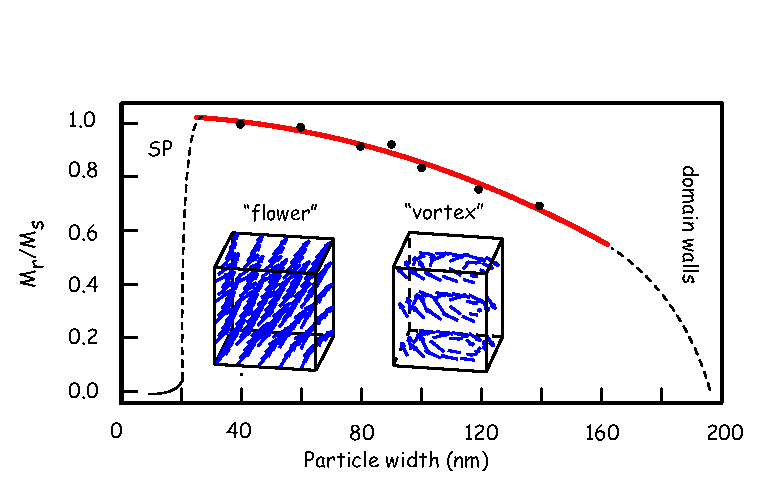
\includegraphics[width=12 cm]{EPSfiles/micromag.eps}
\caption{Possible non-uniform magnetization configurations that reduce self energy for magnetite with increasing particle widths.  The net remanent magnetization reduces with increasingly non-uniform spin configurations.    [Data from Tauxe et al., 2002.]}
\label{fig:nonuniform}
\end{figure}
\nocite{tauxe02}



\subsection{Magnetic energy and magnetic stability}
\label{sect:coercivity}

 Paleomagnetists worry about how long a magnetization can remain fixed within a particle and we will begin to discuss this issue later in the chapter.  It is worth pointing out here that any discussion of magnetic stability will involve magnetic anisotropy energy because this controls the energy required to change a magnetic moment from one easy axis to another.      One way to accomplish this change is to apply a magnetic field sufficiently large that its magnetic energy exceeds the  anisotropy energy.  The magnetic field  capable of flipping the magnetization of an individual uniformly magnetized particle (at saturation, or  $M_s$) over the magnetic anisotropy energy barrier  is the
 \index{coercivity!microscopic}
 \index{magnetic!anisotropy energy!cubic}
  {\it microscopic coercivity} $H_k$.  For uniaxial anisotropy ($K=K_u$) and for cubic magnetocrystalline  anisotropy ($K=K_1$), 
 microscopic coercivity is  given by:
 
\begin{equation}
 H_k = {{ 2 K_u}\over {\mu_oM}}   = { {4\over 3}}{ { |K_1|}\over {\mu_o M_s}}.  
\label{eq:Bk}
\end{equation}

\noindent  respectively (see
\index{Dunlop, D.J.}
\index{\"Ozdemir, \"O.}
\nocite{dunlop97}
Dunlop and \"Ozdemir, 1997 for a more complete derivation).   For elongate particles dominated by shape anisotropy,   $H_k$ reduces to  $  \Delta NM$.  [Note that the units for coercivity as derived here are in Am$^{-1}$, although they are often measured using instruments calibrated in tesla.   Technically,  because the field doing the flipping is inside the magnetic particle and $\B$ (measured in tesla) depends on the magnetization $\M$ as well as the field $\H$ (Equation~\ref{eq:B}), coercivity should be written as $\mu_o H_k$ if the units are quoted in tesla. Microscopic coercivity is another parameter with many names: 
\index{flipping!field}
\index{coercivity}
{\it flipping field}, {\it switching field}, {\it intrinsic coercivity} and also more loosely,   the  {\it coercive field} and {\it coercivity}. We will come back to the  topic of coercivity in Chapter 5.  ]


\begin{figure}[h!tb]
%\epsfxsize 14cm
%\centering \epsffile{EPSfiles/domains.eps}
\centering  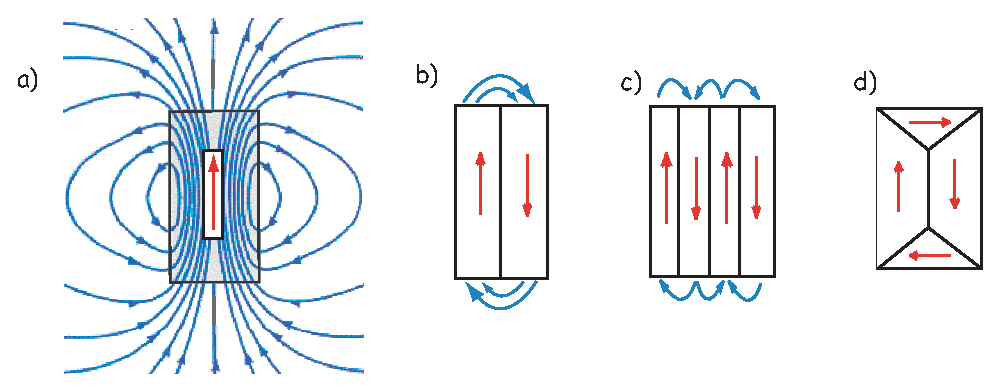
\includegraphics[width=14 cm]{EPSfiles/domains.eps}
\caption{A variety of domain structures of a given particle.  a) Uniformly magnetized (single domain).   [Adapted from Tipler, 1999.] b) Two domains.  c) Four domains in a lamellar pattern.  d) Essentially two domains with two closure domains.}
\label{fig:domains}
\end{figure}
\nocite{tipler99}



\section {Magnetic domains}


So far we have  been discussing hypothetical magnetic particles that are uniformly magnetized. Particles with strong magnetizations (like magnetite) have self energies that quickly become quite large because of the dependence on the square of the magnetization.   We have been learning about several mechanisms that tend to align magnetic spins. In fact in very small particles of magnetite ($<$ 40 nm), the  spins are essentially lined up.  The particle is uniformly magnetized  and we called it single domain (SD).  In larger particles  ($\sim$80 nm) the self energy exceeds the other exchange and magnetocrystalline energies and  crystals  have distinctly non-uniform states of magnetization.   


There are many strategies possible for magnetic particles to reduce self energy.    Numerical models (called {\it micromagnetic models}) can find internal magnetization configurations that minimize the energies discussed in the preceding sections.  
\index{micromagnetic modeling}
Micromagnetic simulations for magnetite particles 
\nocite{schabes88}
\index{Schabes, M.E.}
\index{Bertram, H.N.}
(e.g. Schabes and Bertram, 1988)  allow us to peer into the state of magnetization inside magnetic particles.  These simulations give a picture of increasing complexity from  so-called 
\index{flower remanent state}
\index{vortex remanent state}
{\it flower} to {\it vortex} (Figure~\ref{fig:nonuniform}) remanent states.  These particles share many properties of the uniformly magnetized single domain particles and are called 
\index{pseudo-single domain}
{\it pseudo-single domain} (PSD) particles.  




As particles grow larger ($>\sim$200 nm), they break into multiple 
\index{magnetic!domains}
magnetic domains,  separated by narrow zones of rapidly changing spin directions called
\index{magnetic!domain walls}
 {\it domain walls}.   Magnetic domains can take many forms.  We illustrate a few in Figure~\ref{fig:domains}. The uniform case (single domain) is shown in  Figure~\ref{fig:domains}a.  The external field is very large because the free poles are far apart (at opposite ends of the particle).   When the particle organizes itself into two domains (Figure~\ref{fig:domains}b), the external field is reduced by about a factor of two.  In the case of four lamellar domains (Figure~\ref{fig:domains}c), the external field is quite small.  The introduction of {\it closure domains} as in Figure~\ref{fig:domains}d reduces the external field to nothing.  

\begin{figure}[htb]
%\epsfxsize 14.5cm
%\centering \epsffile{EPSfiles/wall.eps}
\centering  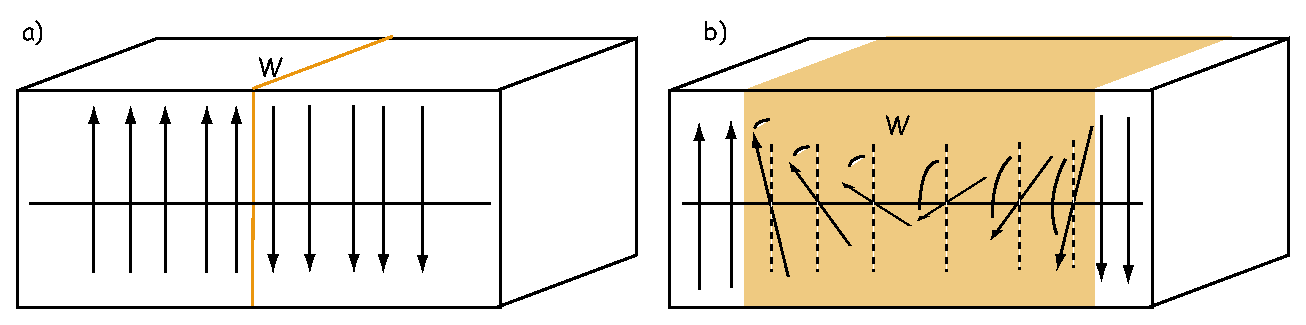
\includegraphics[width=14.5 cm]{EPSfiles/wall.eps}
\caption{Examples of possible domain walls.  a) There is a 180$^{\circ}$ switch from one atom to the next.  The domain wall is very thin, but the exchange price is very high.  b) There is a more gradual switch from one direction to the other [note: each arrow represents several 10's of unit cells].  The exchange energy price is lower, but there are more spins in unfavorable directions from a magnetocrystalline point of view.  }
\label{fig:wall}
\end{figure}
%\eject



As you might already suspect, domain walls are not  ``free'', energetically speaking.  If, as in Figure~\ref{fig:wall}a, the spins simply switch from one orientation to the other abruptly,  the exchange energy cost would be very high.  One way to get around this  to spread the change over several hundred atoms, as sketched in Figure~\ref{fig:wall}b.  The wall width $\delta$ is wider and the exchange energy price is much less.  However, there are now spins in unfavorable directions from a magnetocrystalline point of view (they are in ``hard'' directions).   Exchange energy therefore favors wider domain walls while magnetocrystalline anisotropy favors thin walls.    With some work (see e.g.,  \index{Dunlop, D.J.}
\index{\"Ozdemir, \"O.}
\nocite{dunlop97}
Dunlop and \"Ozdemir, 1997, pp. 117-118), it is possible to come up with the following analytical expressions for wall width ($\delta_w$) and 
\index{magnetic!domain walls!energy}
wall energy density  ($\epsilon_w$):

\beq
\delta_w = \pi {\bigl( {A\over K} \bigr)}^{1\over 2},  \epsilon_w = 2\pi (AK)^{1\over 2},
\label{eq:wall}
\eeq
\noindent where $A$ is the 
\index{magnetic!energy!exchange!constant}
exchange constant  (see Section~\ref{sect:exchange}) and $K$ is the magnetic anisotropy constant (e.g., $K_u$ or $K_1$).   Note that $\epsilon_w$ is the energy density per unit wall area, not per volume.    Plugging in values for magnetite given previously we get $\delta_w$ = 90 nm and $\epsilon_w$  = 3x 10$^{-3}$Jm$^{-2}$.    



In Figure~\ref{fig:energies} we plot the 
\index{magnetic!self energy}
self energy (Equation~\ref{eq:self})  and the wall energy ($\epsilon_w$ from Equation~\ref{eq:wall}) for spheres of magnetite.  We see that the wall energy in  particles with diameters of some 50 nm  is less than the self energy, yet the width of the walls about twice as wide as that.  So the smallest wall is really more like the vortex state and it is only for particles larger than a few tenths of a micron that true domains separated by discrete walls can form.   Interestingly, this is precisely what is predicted from micromagnetic modelling (e.g., Figure~\ref{fig:nonuniform}).   


\begin{figure}[htb]
%\epsfxsize 9.5cm
%\centering \epsffile{EPSfiles/energies.eps}
\centering  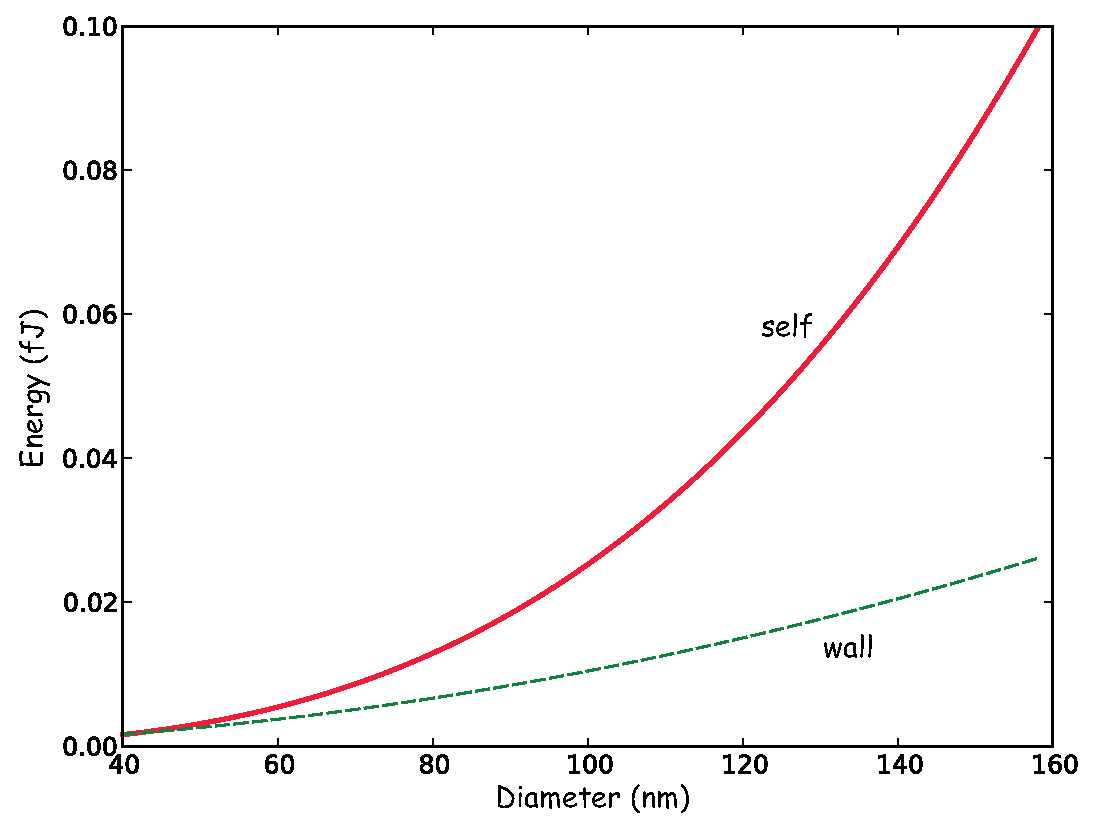
\includegraphics[width=9.5 cm]{EPSfiles/energies.eps}
\caption{Comparison of ``self'' energy versus the energy of the domain wall in magnetite spheres as a function of particle size.}
\label{fig:energies}
\end{figure}



How can we test the theoretical predictions of domain theory?  Do domains really exist?  Are they the size and shape we expect?  Are there as many as we would expect?    In order to address these questions we require a way  of imaging magnetic domains.  
\index{Bitter, F.}
Bitter (1931) \nocite{bitter31} devised a way for doing just that.  Magnetic domain walls are regions with large stray fields (as opposed to domains in which the spins are usually parallel to the sides of the crystals to minimize stray fields).  In the
\index{domain imaging!Bitter technique}
 {\it Bitter technique} magnetic colloid material is drawn to the regions of high field gradients on highly polished sections  allowing the domain walls to be observed (see Figure~\ref{fig:domain-images}a).  

\begin{figure}[h!tb]  
%\epsfxsize 11cm
%\centering \epsffile{EPSfiles/domain-images.eps}
\centering  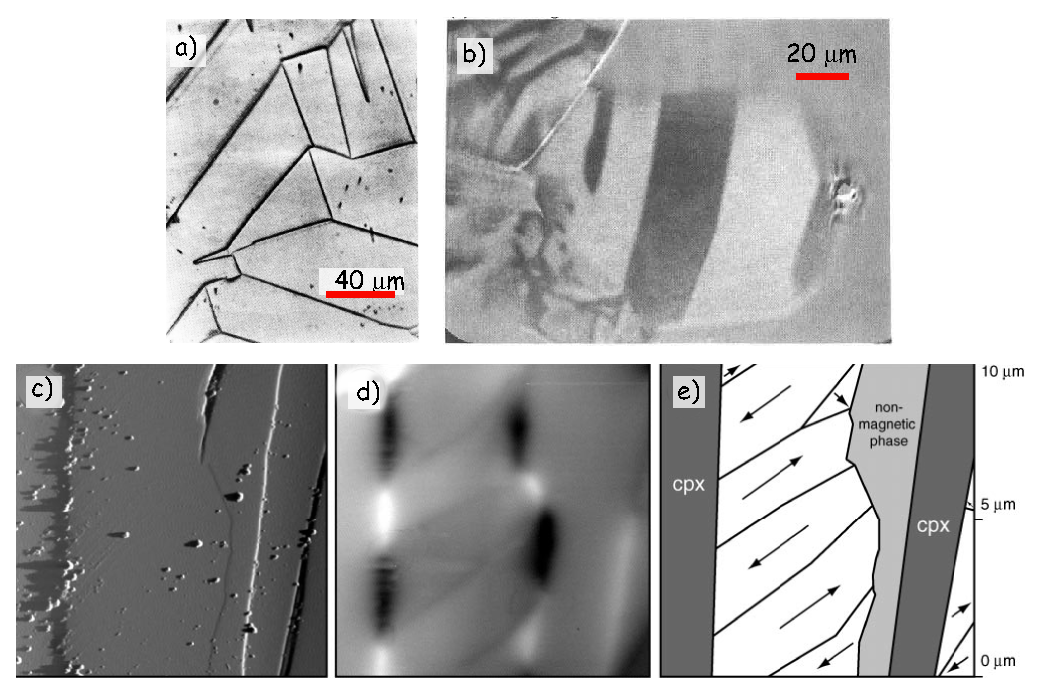
\includegraphics[width=11 cm]{EPSfiles/domain-images.eps}
\caption{a) Bitter patterns from an oriented polished section of magnetite. [Figure from \"Ozdemir et al., 1995]. b) Domains revealed by longitudinal magneto-optical Kerr effect. [Image from Heider and Hoffmann, 1992.]  c-e)  Magnetic force microscopy technique. [Images from Feinberg et al., 2005.] c) Image of topography of surface of a magnetite inclusion in a non-magnetic matrix.  d) Magnetic image from MFM techqnique.  e) Interpretation of magnetizations of magnetic domains.   }
\label{fig:domain-images}
\end{figure}
\nocite{feinberg05}  \nocite{heider92} \nocite{ozdemir95}

There are by now other ways of imaging magnetic domains.  We will not review them all here, but will just highlight the ways that are more commonly used in rock and paleomagnetism.  The
\index{domain imaging!magneto-optical Kerr effect} 
{\it magneto-optical Kerr effect}  or MOKE  uses the interaction between polarized light and the surface magnetic field of the target.   The light interacts with the magnetic field of the sample which causes a small change in the light's polarization and ellipticity.   The changes are detected by reflecting the light into nearly-crossed polarizers.   The longitudinal Kerr effect can show the alignment of magnetic moments in the surface plane of the sample. Domains with different magnetization directions show up as lighter or darker regions in the MOKE image (see Figure~\ref{fig:domain-images}b.) 


Another common method for imaging magnetic domains employs a technique known as 
\index{domain imaging!magnetic  force microscopy}
{\it magnetic force microscopy}.  
Magnetic force microscopy (MFM) uses a scanning probe microscope that maps out the vertical component of the magnetic fields produced by a highly polished section.   The measurements are made with a cantilevered magnetic tip that responds to the magnetic field of the sample.  In practice, the measurements are made in two passes.  The first establishes the topography of the sample (Figure~\ref{fig:domain-images}c).  Then in the second pass, the tip is raised slightly above the surface and by subtracting the �topographic only� signal the attraction of the magnetic surface can be mapped (Figure~\ref{fig:domain-images}d).   Figure~\ref{fig:domain-images}e shows an interpretation of the magnetic directions of different magnetic domains.  



\section{Thermal energy}
\label{sect:tau}

\index{thermal energy}
We have gone some way toward answering the questions posed at the beginning of the chapter. We see now that  anisotropy energy, with contributions from crystal structure, shape and stress, that inhibits changes in the magnetic direction thereby offering a possible mechanism whereby a given  magnetization could be preserved for posterity.  We also asked the question of what allows the magnetization to come into equilibrium with the applied magnetic field in the first place;  this question requires a little more work to answer.  The key to this question is to find some mechanism which allows the moments to ``jump over'' magnetic anisotropy energy barriers.   One such mechanism is  thermal energy $E_T$, which was given in Chapter 3 as:

$$
E_T = kT.
$$

We know from statistical mechanics that the probability $P$ of finding a grain with a given thermal energy  sufficient to overcome some anisotropy energy $E_a$ and change from one easy axis to another is $P=\exp (-E_a/E_T )$.   Depending on the temperature,  such grains may be quite rare, and we may have to wait some time $t$ for a particle to work itself up to jumping  over the energy barrier.  


\begin{figure}[htb]
%\epsfxsize 10cm
%\centering \epsffile{EPSfiles/tauvd.eps}
\centering  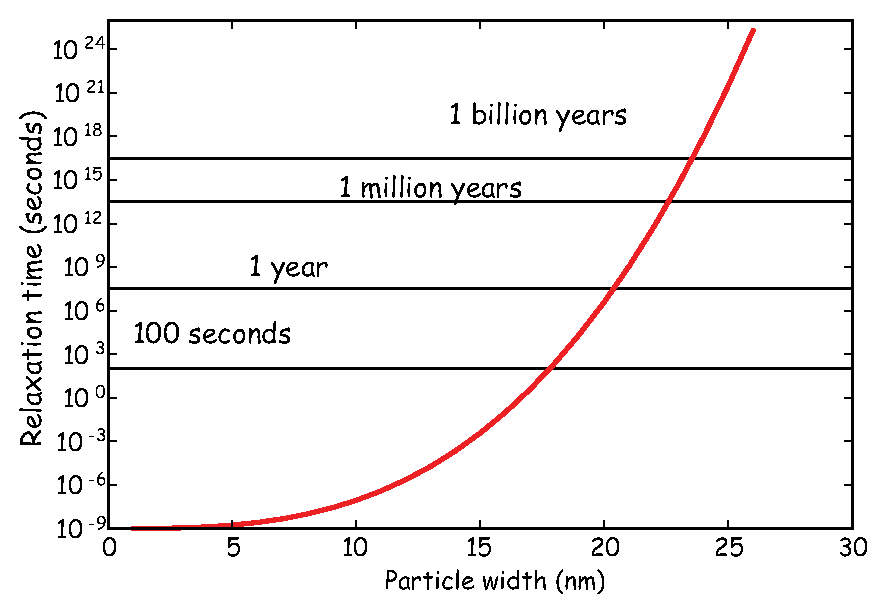
\includegraphics[width=9.5 cm]{EPSfiles/tauvd.eps}
\caption{Relaxation time in magnetite ellipsoids as a function of grain width in nanometers (all length to width ratios of 1.3:1.)  }
\label{fig:tauvd}
\end{figure}
 


Imagine a block of material containing a random assemblage of magnetic particles that are for simplicity uniformly magnetized  and dominated by uniaxial anisotropy.  Suppose that this block has some initial magnetization $M_o$ and is placed in an environment with no ambient magnetic field.  Anisotropy energy will tend to keep each tiny magnetic moment in its original direction and the magnetization will not change over time.  At some temperature,  certain grains will have sufficient energy to overcome the anisotropy energy and flip their moments to the other easy axis.   As the energy surface is spherical, with no dimples or protruberances, there is no preferred direction and, over time, the magnetic moments will become random.  
Therefore, the magnetization as a function of time in this simple scenario will decay to zero.  The equation governing this decay is:  

\begin{equation}
M(t) = M_o \exp ({-t\over {\tau}}),
\label{eq:MvT}
\end{equation}

\noindent where $t$ is time and $\tau$ is an empirical constant called the {\it relaxation time}.  Relaxation time is   the time required for the remanence to decay to $1/e$ of $M_o$.    This equation is the essence of what is called
\index{N\'eel!theory}
\index{N\'eel, L.}
{\it N\'eel theory}
  \nocite{neel55} 
  (see, e.g., N\'eel, 1955).
\index{relaxation time}
The value of $\tau $ depends on the  competition between 
magnetic anisotropy energy and 
thermal energy.  It is a measure of the probability that a grain will have
sufficient thermal energy to overcome the anisotropy energy and switch its
moment.  Therefore in zero external field:

\begin{equation}
{\tau } = {{1\over C} \exp
{[{\hbox{anisotropy}\hskip 1em \hbox{energy}}]\over
[{\hbox{thermal }\hskip 1em \hbox{energy}}]}} =
{{1\over C} \exp {[K v]\over [kT]}},
\label{eq:tau}
\end{equation}

\noindent where $C$ is a 
frequency factor with a value of something like
$10^{10}$ s$^{-1}$.  The anisotropy energy is given by the dominant 
anisotropy parameter $K$ (either $K_u, K_1$, or $\lambda$)
 times the grain volume $v$.  
 
\index{thermal energy}%

Thus,  the 
\index{relaxation time}%
relaxation time is proportional to anisotropy constant and 
volume, and is inversely related to
temperature.
\index{relaxation time}%
Relaxation time $\tau $ varies  rapidly with small changes in $v$ and $T$.
To see how this works, we can take $K_u$ for slightly elongate cuboids of  magnetite (length to width ratio of 1.3 to 1)  and evaluate relaxation time as a function of particle width (see Figure~\ref{fig:tauvd}).   There is a sharp transition between grains with virtually no stability
($\tau $ is on the order of seconds) and grains with stabilities of billions of years. 

Grains with $\tau \simeq 10^2 - 10^3$ seconds have sufficient thermal energy
to overcome the anisotropy energy frequently and are unstable on a laboratory
time scale.  In zero field, these grain moments will tend to rapidly
become random,  and
in an applied field, also tend to align  rapidly with the field.  
The net magnetization is related to the field by a
Langevin function (see Section~\ref{sect:para} in Chapter 3).  Therefore, this
 behavior is quite similar to paramagnetism, hence these grains are called 
\index{superparamagnetism}%
{\it superparamagnetic} (SP). Such grains can be distinguished from paramagnets,
however, because the field required to saturate the moments is typically much
less than a tesla, whereas that for paramagnets can exceed hundreds of
tesla. 

\begin{figure}[h!tb]
%\epsfxsize 9.5cm
%\centering \epsffile{EPSfiles/butban.eps}
\centering  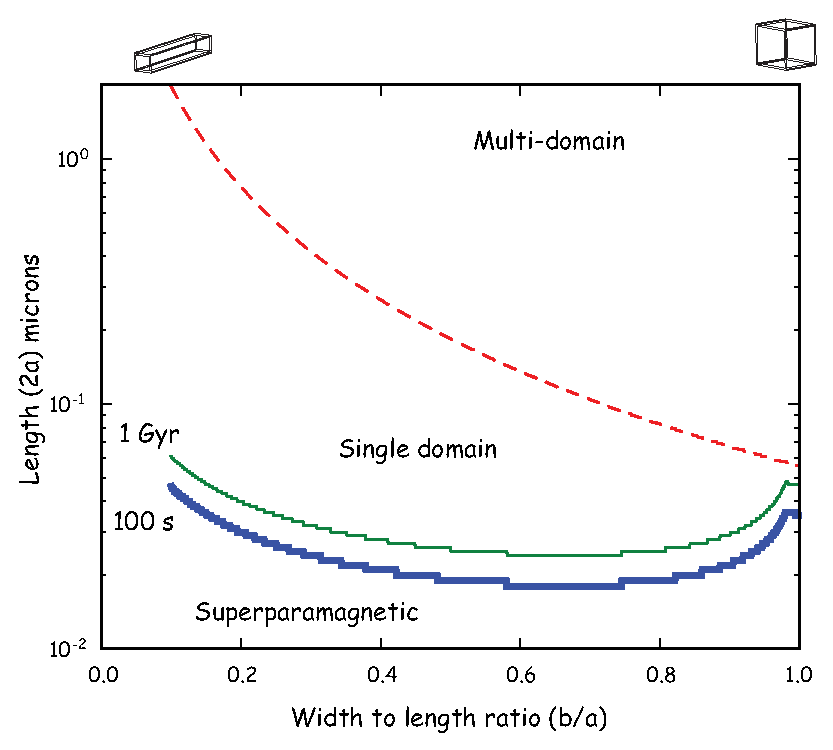
\includegraphics[width=9.5 cm]{EPSfiles/butban.eps}
\caption{ Expected domain states for various sizes and shapes of  parallelopipeds of magnetite at room temperature.  The parameters $a$ and $b$ are as in Figure 4.4e.  Heavy blue (thin green) line is the superparamagnetic threshold assuming a relaxation time of 100s (1 Gyr).   Dashed red line marks the SD/MD threshold size.  Calculations done using assumptions and parameters described in the text.  }
\label{fig:butban}
\end{figure}


\section{Putting it all together}


We are now in a position to pull together all the threads we have considered in this chapter and make a plot of what sort of magnetic particles behave as superparamagnets, which should be single domain and which should be multi-domain according to our simple theories.   We can estimate the superparamagnetic to single domain threshold for magnetite as a function of particle shape by finding for the length (2a) that gives a relaxation time of 100 seconds as a function of width to length ratio ($b/a$) for parallelopipeds of magnetite (heavy blue line in  Figure~\ref{fig:butban}).    To do this, we  follow the logic of  
\index{Evans, M.E.}
\index{McElhinny, M.W.}
Evans and McElhinny (1969) \nocite{evans69} and 
\nocite{butler75}  
\index{Butler, R.F.}
\index{Banerjee, S.K.}
 Butler and Banerjee (1975).   In this 
\index{diagrams!Evans}
{\it Evans diagram}, we estimated relaxation time using  Equation~\ref{eq:tau},  plugging in  values of $K$ as either the magnetocrystalline effective anisotropy constant (${1\over{12}}K_1$) or the shape anisotropy constant (${1\over 2} \Delta N \mu_o M^2$), whichever was less.   We also show the curve at which relaxation time is equal to 1 Gyr, reinforcing the point that very small changes in crystal size and shape make profound differences in relaxation time.     
The figure also predicts the boundary between the single domain field and the two domain field,  when the energy of a domain wall is less than the self energy of a particle that is uniformly magnetized.  This can be done by evaluating wall energy with Equation~\ref{eq:wall} for a wall along the length of a parallelopiped and area ($4ab$) as compared to the self energy (${1\over 2} \mu_o N_a M^2v$) for a given length and width to length ratio.  When the wall energy is less than the self energy, we  are in the two domain field.    




Figure~\ref{fig:butban} suggests that there is virtually no SD stability field for equant magnetite; particles are either SP or MD (multi-domain).  As the width to length decreases (the particle gets longer), the stability field for SD magnetite expands.  Of course micromagnetic modelling shows that there are several transitional states between uniform magnetization (SD) and MD, i.e. the flower and vortex remaent states (see 
\nocite{fabian96} 
\index{Fabian, K.L.}
Fabian et al., 1996), but Figure~\ref{fig:butban} has  enormous predictive power and the version of 
\nocite{butler75}  
\index{Butler, R.F.}
\index{Banerjee, S.K.}
Butler and Banerjee (1975), (which is slightly different in detail)  continues to be used extensively.    It is worth pointing out however, that the size at which domain walls appear in magnetite is poorly constrained because it depends critically on the exact shape of the particle,  its state of stress and even its history of exposure to past fields.  Estimates in the literature range from as small as 20 nm  to much larger (up to 100 nm) depending on how the estimates are made.   Nonetheless, it is probably true that truly single domain magnetite is quite rare in nature, yet more complicated states are difficult to treat theoretically.   Therefore most paleomagnetic studies rely on predictions made for single domain particles.


\noindent{SUPPLEMENTAL READING:} Dunlop and \"Ozdemir (1997), Chapters 2.8 and 5.



\section{Problems}

{\parindent 0pt \parskip 12pt 

{\bf Problem 1}

Assume that the magnetization of magnetite is about 480 mAm$^{-1}$ and using values for other parameters from the text,  write a Python program to calculate  the following:

a) Self energy (or magnetostatic energy) for a sphere 1, 10 and 100 $\mu$m in diameter. [Hint: see Equation~\ref{eq:self}  in the text for the `self' energy density. Also, remember the difference between energy and energy density!] 

b) Magnetostatic (shape) anisotropy energy for an ellipsoid whose principal semi-axis is 1 $\mu$m and whose major and minor semi-axes are each 0.25 $\mu$m.  You may use the ``nearly spherical'' approximation in the text.   

c) The critical radius of a sphere at which wall energy equals self energy.


{\bf Problem 2}

Calculate  grain diameter for magnetite spheres with $\tau$s of 10$^{-1}$, 10, 10$^2$, 10$^3$, 10$^5$, 10$^9$, 10$^{15}$ seconds.  Use values for Boltzmann's constant, $C$ (the frequency factor) and $|K_1|$ at room temperature (300K).    

{\bf Problem 3}

Consider a highly elongate rod (needle-shaped grain) of ferromagnetic material.

a) Explain why the demagnetizing factor along the long axis of the rod is about zero and about one half across the axis.

b)  For a needle shaped grain of magnetite ($M_s=4.8\cross 10^5$ Am$^{-1}$), what external magnetic field is required to magnetize the rod to saturation along the diameter (perpendicular to the long axis)?

c) What is the maximum microscopic coercivity of magnetite (assume an infinitely long grain)?  
}



%http://www-physique.u-strasbg.fr/~udp/articles/chimie/weblab.htm

%http://www.ontariominerals.com/magnetite.htm

%http://www.gly.uga.edu/schroeder/geol3010/magnetite.gif

%http://www.geo.umn.edu/orgs/irm/bestiary/index.html

